\section*{Rechenaufwand (n-Körper Problem)}

\begin{equation}
  O(n) = n^2 \quad \Rightarrow \quad O(n) = n \cdot log(n)
\end{equation}

Um die Kräfte die zwischen allen Sternen in einer Galaxie wirken zu berechnen
werden \( n^2 \) Rechenschritte benötigt (\( n \) entspricht der Anzahl der)
Sterne.

\vspace{-0.25cm}
\begin{center}
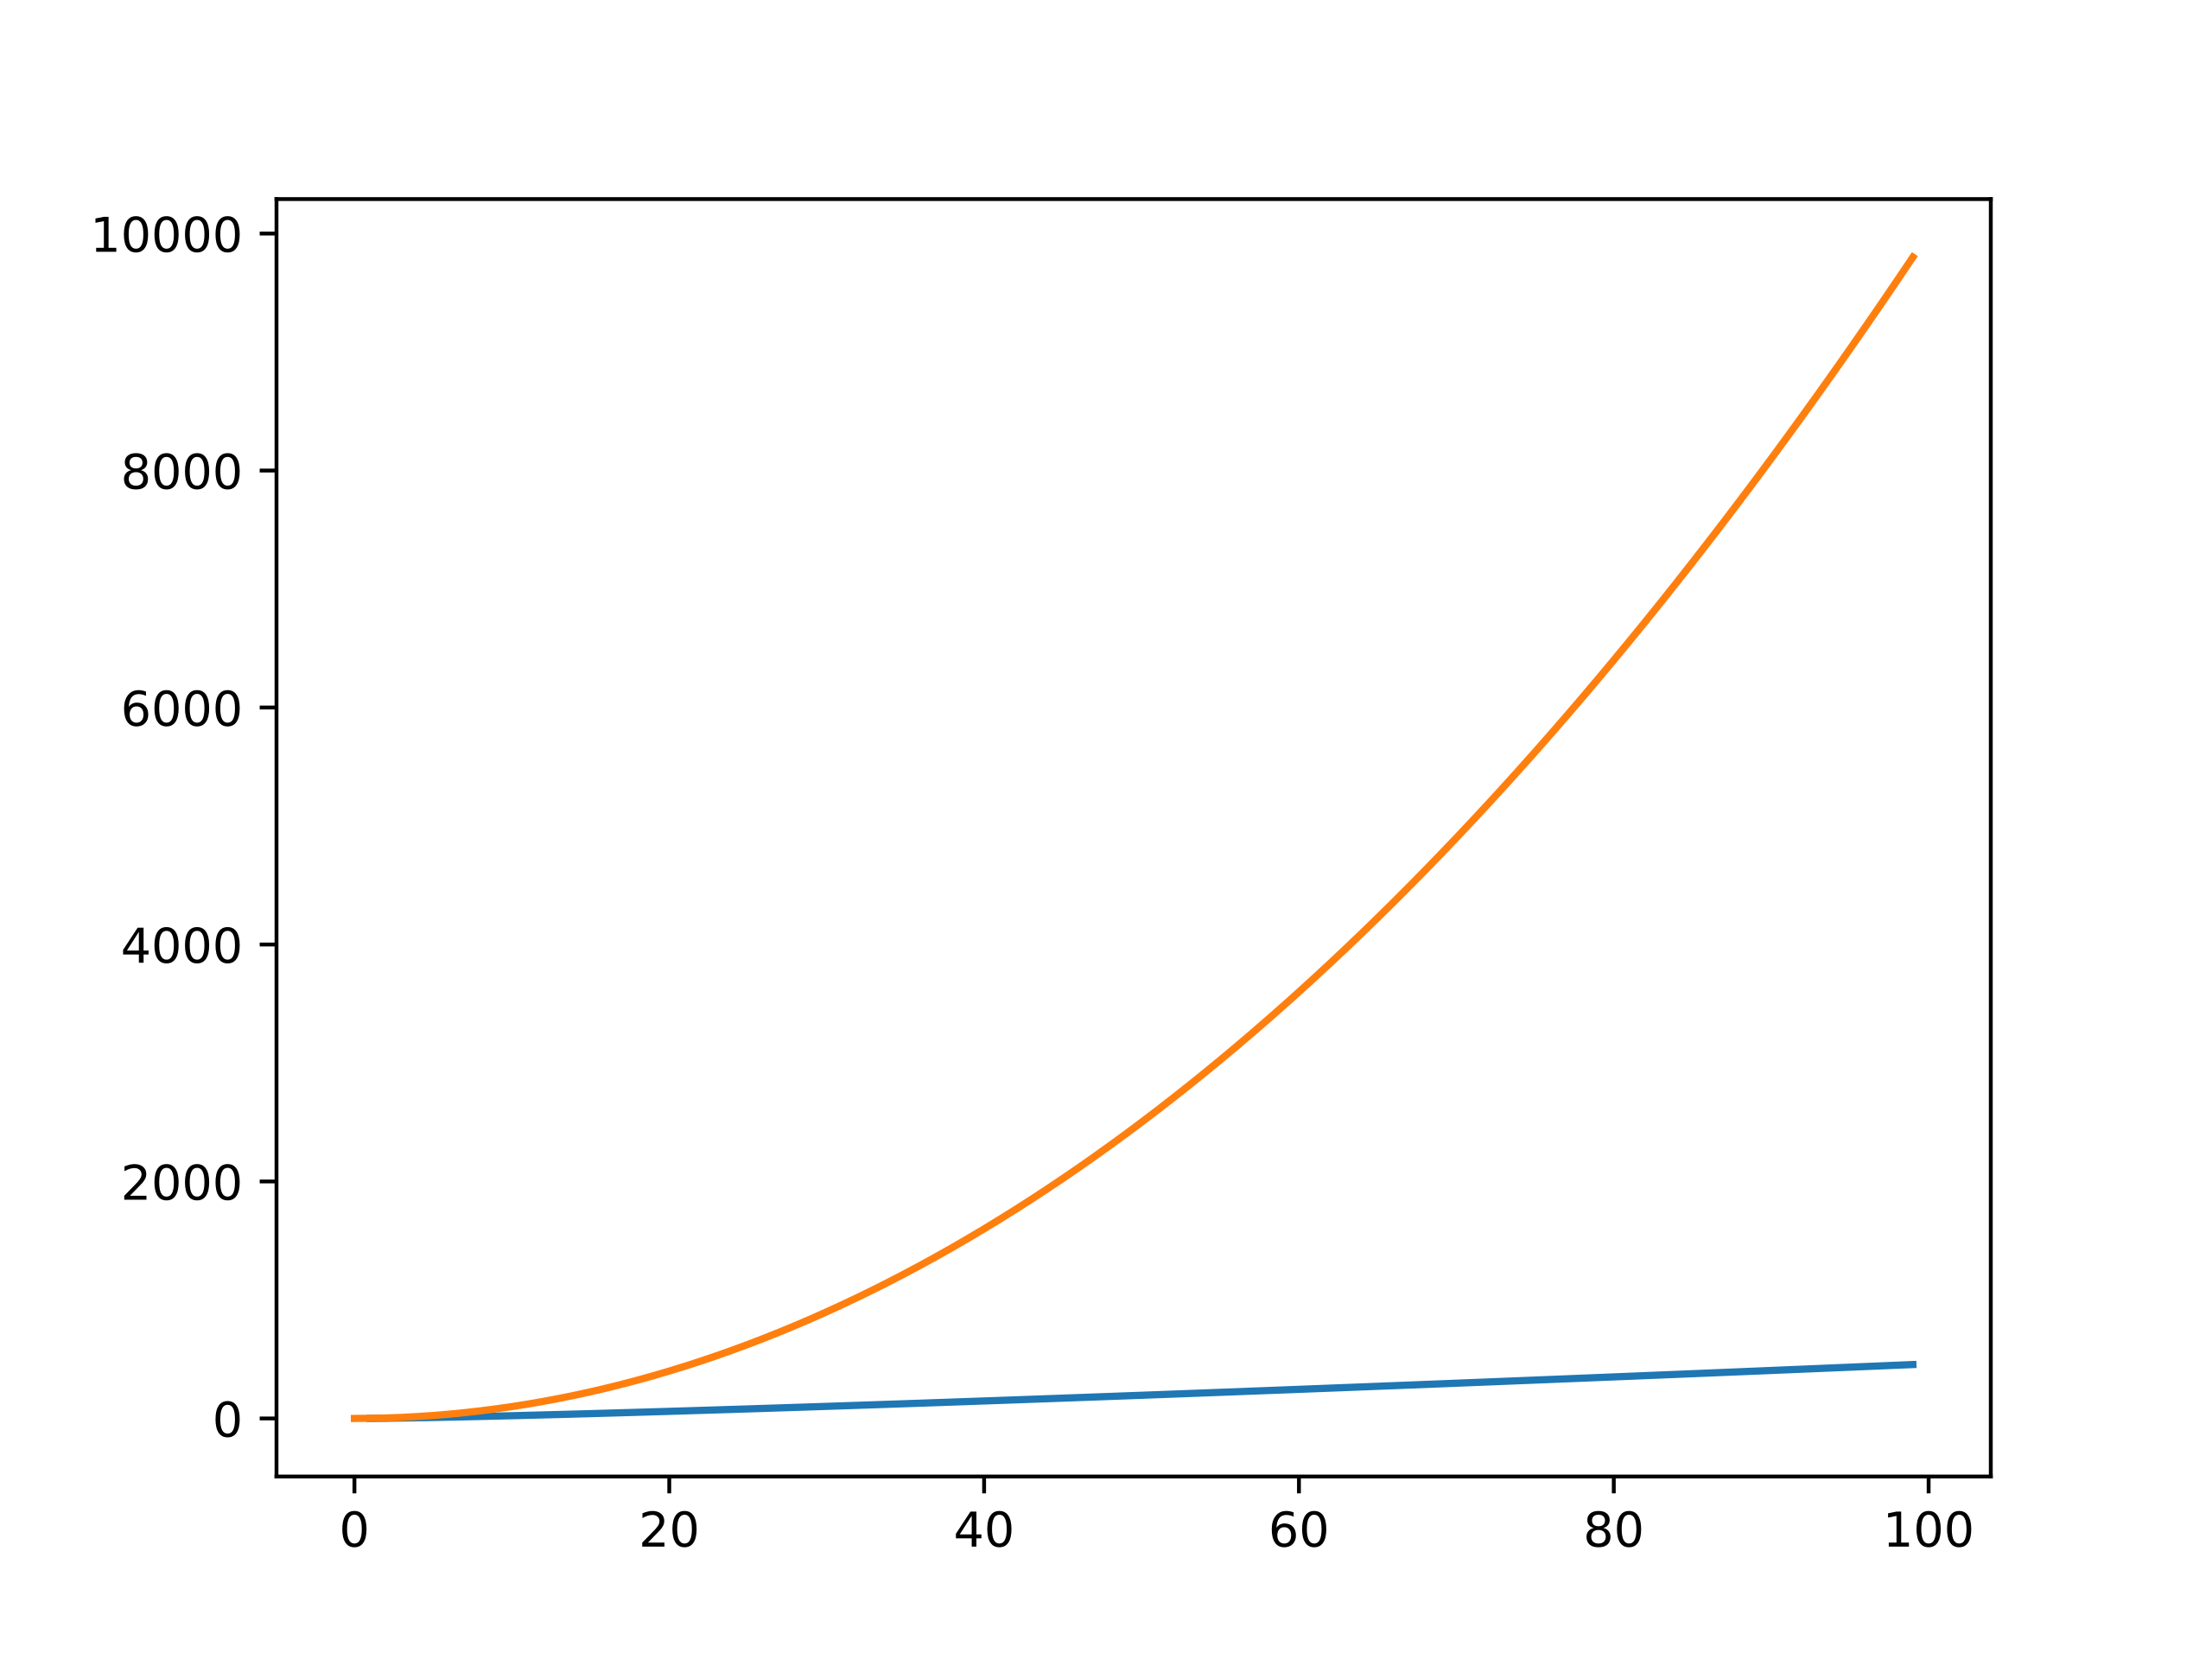
\includegraphics[width=0.8\linewidth]{figs/bigo_large}
\caption{Orange \( n^2 \), Blau \( n \log(n) \)}
\label{fig:bigo}
\end{center}\vspace{-1.25cm}
